\documentclass[
oneside,
a4paper,
12pt,
titlepage]
{article}
\usepackage[english]{babel}

\input{/home/renke/Uni/Formatvorlagen/LaTeX/packages.tex}
\input{/home/renke/Uni/Formatvorlagen/LaTeX/settings.tex}
\input{/home/renke/Uni/Formatvorlagen/LaTeX/settings_article.tex}
\input{/home/renke/Uni/Formatvorlagen/LaTeX/settings_bibliography.tex}
\input{/home/renke/Uni/Formatvorlagen/LaTeX/hyphenation_english.tex}

%%%%%%%%%%%%%%%%%%%%%%%%%%%%%%%%%%%%%%%%%%%%%%
%% TikZ settings specific to this document. %%
%%%%%%%%%%%%%%%%%%%%%%%%%%%%%%%%%%%%%%%%%%%%%%
%% Load TikZ libraries.
\usetikzlibrary[shapes.geometric,intersections]
%% Set drawing options for figures.
\tikzset{DataSelectionFlowChartStart/.style = {
    draw,
    shape = circle,
    top color = white,
    bottom color = green!30,
    line width = 0cm,
    trapezium angle = 45,
    align = center}}
\tikzset{DataSelectionFlowChartAction/.style = {
    draw,
    shape = trapezium,
    top color = white,
    bottom color = violet!30,
    line width = 0cm,
    trapezium angle = 45,
    align = center}}
\tikzset{DataSelectionFlowChartQuestion/.style = {
    draw,
    rounded corners,
    shape=diamond,
    top color = white,
    bottom color = violet!30,
    line width = 0cm,
    aspect=2,
    align = center}}
\tikzset{DataSelectionFlowChartResult/.style = {
    draw,
    shape = rectangle,
    fill = white,
    line width = 0cm,
    align = center}}
\tikzset{DataSelectionFlowChartEnd/.style = {
    draw,
    shape = circle,
    top color = white,
    bottom color = red!30,
    line width = 0cm,
    trapezium angle = 45,
    align = center}}
\tikzset{DataSelectionFlowChartArrow/.style = {
    ->,
    thick}}
\tikzset{DataSelectionFlowChartLine/.style = {
    thick}}

\addbibresource[location=local]{../../Literature/MasAr_Literature.bib} % s. S. 71 f. biblatex-Dokumentation

%% AUCTeX style file: ./style/MasAr_Thesis.el

%% Define custom SI units.
\DeclareSIUnit\years{a}

%% Define custom commands.
\newcommand{\beech}[0]{European beech (\emph{Fagus sylvatica} L.)}
\newcommand{\spruce}[0]{Norway spruce (\emph{Picea abies} (L.) H.\textsc{Karst})}
\newcommand{\ponderosa}[0]{Ponderosa pine (\emph{Pinus ponderosa} \textsc{Douglas})}
\newcommand{\refeq}[1]{equation~(\ref{#1})}
\newcommand{\reftab}[1]{Table~\ref{#1}}
\newcommand{\reffig}[1]{Figure~\ref{#1}}

\begin{document}

\begin{titlepage}

\begin{center}

\vspace*{5cm}

{\LARGE Modelling maximum basal area of pure beech and spruce stands in northwestern Germany \\}

\vspace{2cm}

{\large Author: \\ Renke Christian von Seggern \par}

\vspace{2cm}

{\normalsize Master’s Thesis at the \\
  Faculty of Forest Sciences and Forest Ecology, \\
  Georg-August-Universität Göttingen}

\vspace{0.5cm}

{\normalsize Date of submission: \\ ??.??.???? \par}

\vspace{0.5cm}

{\normalsize Supervisors: \\ Prof. Dr. Winfried Kurth \\ Prof. Dr. Jürgen Nagel \par}

\end{center}

\end{titlepage}

%%% Local Variables:
%%% mode: latex
%%% TeX-master: "MasAr_Thesis.tex"
%%% End:

\newpage

\pagestyle{toc}

\pagenumbering{Roman}

{
\renewcommand{\MakeUppercase}[1]{#1} % http://tex.stackexchange.com/questions/179966/fancyhdr-chaptermark-and-table-of-contents

\singlespacing % http://tex.stackexchange.com/questions/56546/how-to-change-spaces-between-items-in-table-of-contents

\tableofcontents

}
%%% Local Variables:
%%% mode: latex
%%% TeX-master: "MasAr_Notes"
%%% End:

\newpage

\pagestyle{standard}
\pagenumbering{arabic}

\pagestyle{abbrevs_symbols}

{
  \renewcommand{\MakeUppercase}[1]{#1} % http://tex.stackexchange.com/questions/179966/fancyhdr-chaptermark-and-table-of-contents

  \newcommand{\mysectiontitle}{Table of abbreviations and symbols} % set section title as a custom macro to ease mutlitple usage (necessary when using a starred sectioning macro)
  
  \section*{\mysectiontitle{}}
  \label{sec:AbbrevsSymbolsTable}
  
  \markboth{\mysectiontitle{}}{} % http://tex.stackexchange.com/questions/89914/chapter-name-in-the-header-with-chapter
  \addcontentsline{toc}{section}{\mysectiontitle{}} % http://tex.stackexchange.com/questions/35433/creating-unnumbered-chapters-sections-plus-adding-them-to-the-toc-and-or-header
  
  % \begin{table}[H]
  %   \centering
  \begin{longtabu}{l L l}
    \toprule
    Symbol & Description & Unit \\
    \midrule
    \endfirsthead
    Symbol & Description & Unit \\
    \midrule
    \endhead
    \bottomrule
    \endlastfoot
    \(D\) & average diameter (by basal area) & \si{\centi\meter} \\
    \(\TopHeight\) & top height, height of dominant trees & \si{\meter} \\
    \(k\) & constant (varying with species) & \\
    log & decadic logarithm & \\
    \(N\) & stand density & \si{\per\hectare} \\
    \(s\) & slope of the \logNlogDcurve{} \\
    \(SI\) & absolute site class & \si{\meter} \\
  \end{longtabu}
  % \end{table}
}

%% Reset table counter.
\setcounter{table}{0}

%%% Local Variables:
%%% mode: latex
%%% TeX-master: "MasAr_Thesis.tex"
%%% End:

\newpage

\section{Selection of data}

\subsection{Maximum basal area and self-thinning}

In his definition of ``maximum basal area'', \textcite{Assmann1970} points out that maximum basal area is only achieved in stands which have not actively been thinned.  In this context, ``active thinning'' means a reduction of stand density exceeding natural density dependent mortality, also known as ``natural thinning'' \parencite{SAF1958} or ``self-thinning'' \parencite{Roehrig1992}.  While self-thinning, by definition, is a naturally occurring phenomenon, the actual cause of thinning, be it inter-plant competition or human influence, is of no relevance to the study at hand as long as the extent of thinning does not exceed natural rates.  Thus, data selection was based on the following rationale: a stand is considered to have maximum basal area, as long as its thinning rate is roughly equal to the self-thinning rate of a stand of the same species.  This, however, requires knowledge of the self-thinning rates of \beech{} and \spruce{}.

\textcite{Reineke1933} proposed that every forest stand, regardless of tree species and stand development, is subject to the same self-thinning rate given by the equation
\begin{equation}
  \label{eq:reineke}
  \log N = s \log D + k ~,
\end{equation}
with \(s = -1.605\).  According to \textcite{Reineke1933}, every increase in the logarithm of mean diameter leads to a \num{1.605}-fold decrease in the logarithm of stand density.

However, the universal applicability of \refeq{eq:reineke} has been called into question.  As an alternative approach, \textcite{Charru2012} proposed the use of a quadratic, rather than a linear logarithmic diameter term in the right hand side of \refeq{eq:reineke}. A similar approach is taken by \textcite{Schuetz2008,Schuetz2010,Zeide1995}, whose results suggested to add a quadratic logarithmic diameter term to the right hand side of \refeq{eq:reineke}.  \textcite{Meyer1938} found that for \ponderosa{}, the line reported by \textcite{Reineke1933} had to be changed to a slightly concave curve in order to fit observations.  

Despite the apparent shortcomings of \refeq{eq:reineke}, its general form has been upheld by other studies.  Building on the findings of \textcite{Drew1979}, \textcite{VanderSchaaf2010,VanderSchaaf2008} argued that \refeq{eq:reineke} is valid, but only during a specific phase of stand development.  Similarly, \textcite{Zeide1985} suggested that \refeq{eq:reineke} is only applicable during the stage of full canopy closure.  A different approach encountered in the literature is to use a species-specific slope rather than the constant of \num{-1.605} reported by \textcite{Reineke1933} \parencite{MacKinney1935,Pretzsch2005,Charru2012,Pretzsch2006,Río2001,Sterba1987,Vacchiano2013,Vospernik2015,Zeide1985,Zeide1987,VanderSchaaf2007}.  See \reftab{tab:SpeciesSpecificReinekeSlopes} for an overview of slopes for \beech{} and \spruce{} as reported in the literature.  \textcite{Pretzsch2000,Pretzsch2002} showed that the rule of \textcite{Reineke1933} may be considered a special case of the \num{-3 / 2} power rule of \textcite{Yoda1963}, claiming that as long as the \num{-3 / 2} power rule is valid, species-specific deviations from Reineke’s constant of \num{-1.605} are a result of species-specific diameter-biomass relationships.

\subsection{Mechanism for selecting maximum stand density-observations}

Considering the current state of research on the topic of self-thinning rates of \beech{} and \spruce{}, an intermediate approach was taken in the present study.  The approach uses \refeq{eq:reineke}, while also incorporating species-specific values for \(s\).  Figure \ref{fig:DataSelectionFlowChart} provides a schematic of the mechanism used for removing those observations belonging to a specific stand which were not considered to be maximum stand density-observations.  In general, the mechanism attempts to answer 2 questions:
\begin{enumerate}
\item Is the slope of \refeq{eq:reineke} between the current and the previous observation greater than or equal to the species-specific lower threshold?
\item Is the slope of \refeq{eq:reineke} between the current and the following observation lower than or equal to the species-specific upper threshold?
\end{enumerate}
An observation is considered to be a maximum stand density-observation if all questions applicable to it are answered positively.  The thresholds were based on literature values and are reported in \reftab{tab:ReinekeSlopeThresholds}.

\newpage{}
\begin{landscape}
  \begin{figure}[h]
    \caption{Flowchart representing the mechanism used for removing observations of a specific stand which were not considered to be maximum stand density-observations based on the slope of \refeq{eq:reineke} between adjacent observations. \\
      \(s_l\): species-specific lower threshold for the slope of \refeq{eq:reineke} (cp. \reftab{tab:ReinekeSlopeThresholds}). \\  %% Note: the hyperlinks in this caption are not placed ontop of the corresponding printed character, but at a seemingly random distance behind it. I am currently (2017-10-03) unsure about the cause of this and thus don’t know of any fix for it.
      \(s_f\): slope of \refeq{eq:reineke} between current and following observation. \\
      \(s_p\): slope of \refeq{eq:reineke} between current and previous observation. \\
      \(s_u\): species-specific upper threshold for the slope of \refeq{eq:reineke} (cp. \reftab{tab:ReinekeSlopeThresholds}).}
    \label{fig:DataSelectionFlowChart}
  {
    \footnotesize
    % \small
    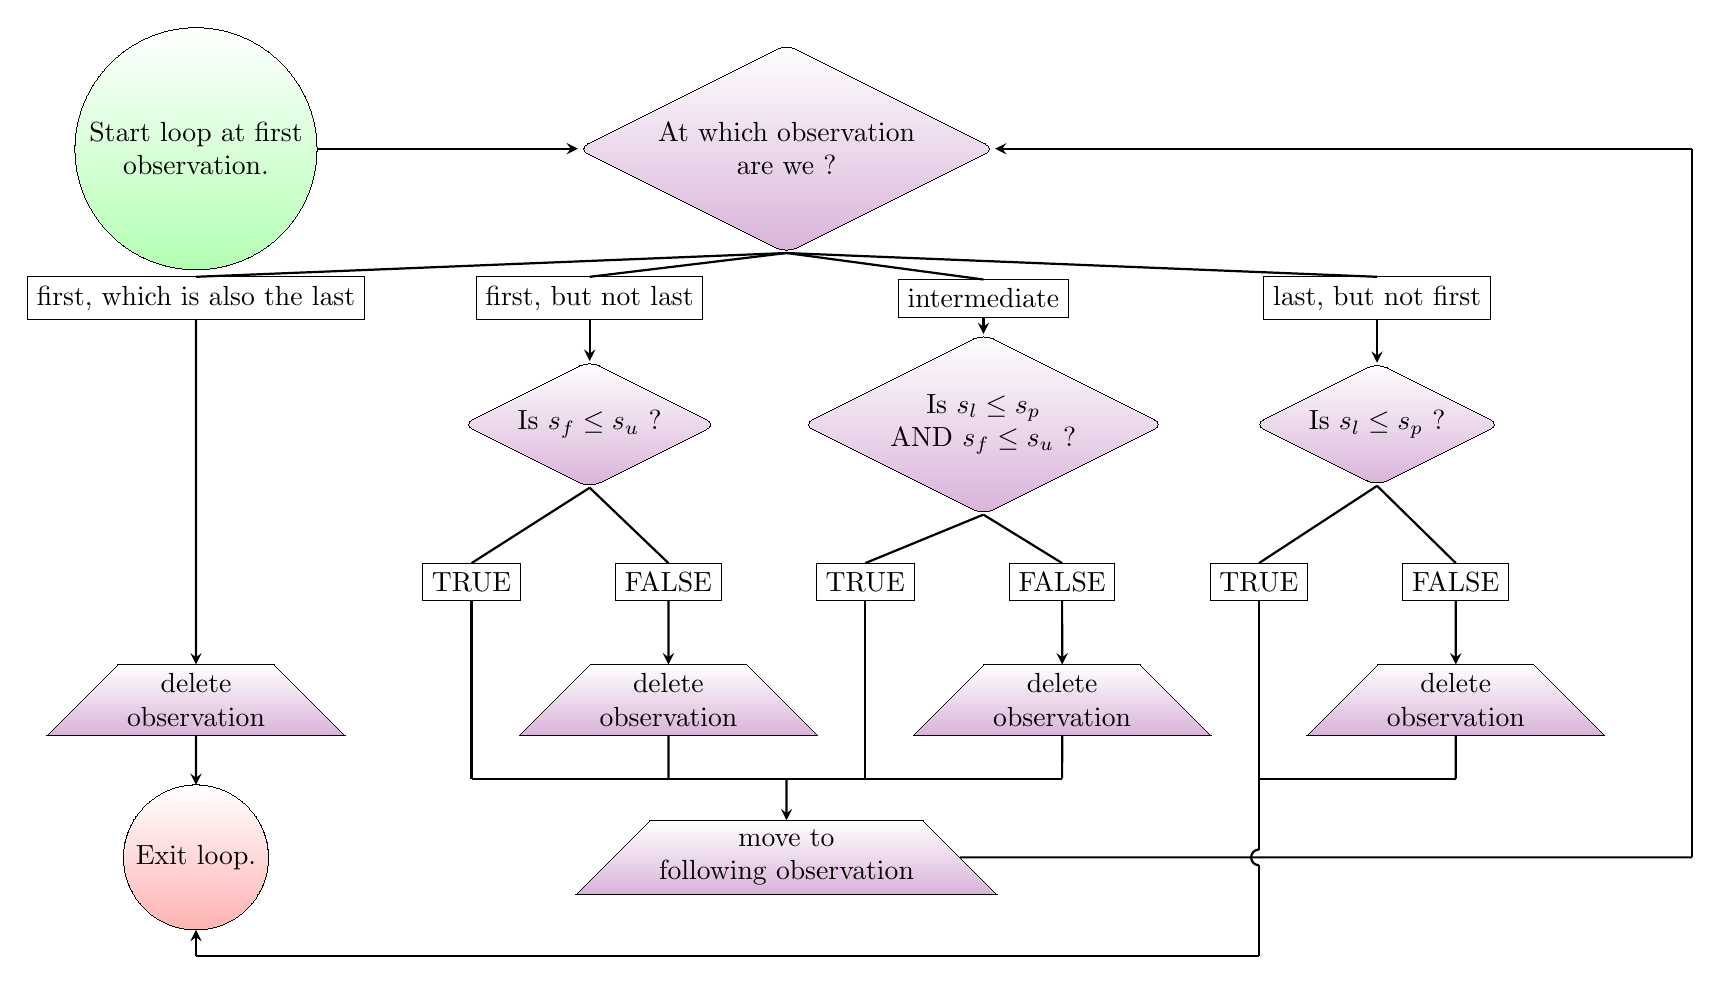
\begin{tikzpicture}[>=stealth,node distance = 0.5]
      %% Start.
      \node (Start1-1) at(0, 0) [DataSelectionFlowChartStart] {Start loop at first \\ observation.};
      %% Questions.
      \node (Question1-1) at(7.5, 0) [DataSelectionFlowChartQuestion] {At which observation \\ are we~?};
      \node (Question2-1) at(5, -3.5) [DataSelectionFlowChartQuestion] {Is \(s_f \leq s_u\)~?};
      \node (Question2-2) at(10, -3.5) [DataSelectionFlowChartQuestion] {Is \(s_l \leq s_p\) \\ AND \(s_f \leq s_u\)~?};
      \node (Question2-3) at(15, -3.5) [DataSelectionFlowChartQuestion] {Is \(s_l \leq s_p\)~?};
      %% Actions.
      \node (Action1-1) at(0,-7) [DataSelectionFlowChartAction] {delete \\ observation};
      \node (Action1-2) at(6,-7) [DataSelectionFlowChartAction] {delete \\ observation};
      \node (Action1-3) at(11,-7) [DataSelectionFlowChartAction] {delete \\ observation};
      \node (Action1-4) at(16,-7) [DataSelectionFlowChartAction] {delete \\ observation};
      \node (Action2-1) at(7.5, -9) [DataSelectionFlowChartAction] {move to \\ following observation};
      %% Results (drawn last because they should cover any lines with which they overlap).
      \node (Result1-1) at(0, -1.9) [DataSelectionFlowChartResult] {first, which is also the last};
      \node (Result1-2) at(5, -1.9) [DataSelectionFlowChartResult] {first, but not last};
      \node (Result1-3) at(10, -1.9) [DataSelectionFlowChartResult] {intermediate};
      \node (Result1-4) at(15, -1.9) [DataSelectionFlowChartResult] {last, but not first};
      \node (Result2-1) at(3.5, -5.5) [DataSelectionFlowChartResult] {TRUE};
      \node (Result2-2) at(6, -5.5) [DataSelectionFlowChartResult] {FALSE};
      \node (Result2-3) at(8.5, -5.5) [DataSelectionFlowChartResult] {TRUE};
      \node (Result2-4) at(11, -5.5) [DataSelectionFlowChartResult] {FALSE};
      \node (Result2-5) at(13.5, -5.5) [DataSelectionFlowChartResult] {TRUE};
      \node (Result2-6) at(16, -5.5) [DataSelectionFlowChartResult] {FALSE};
      %% End.
      \node (End1-1) at(0, -9) [DataSelectionFlowChartEnd] {Exit loop.};
      %% Horizontal lines and arrows.
      \draw [DataSelectionFlowChartArrow] (Start1-1.east) -- (Question1-1.west); \draw [DataSelectionFlowChartArrow] (19, 0) -- (Question1-1.east);
      \draw [DataSelectionFlowChartLine] (3.5, -8) -- (11, -8); \draw [DataSelectionFlowChartLine] (13.5, -8) -- (16, -8);
      \draw [DataSelectionFlowChartLine] (Action2-1.east) -- (19, -9);
      \draw [DataSelectionFlowChartLine] (13.5, -10.25) -- (0, -10.25);
      %% Vertical lines.
      \draw [DataSelectionFlowChartArrow] (Result1-1.south) -- (Action1-1.north); \draw [DataSelectionFlowChartArrow] (Action1-1.south) -- (End1-1.north); \draw [DataSelectionFlowChartArrow] (0, -10.25) -- (End1-1.south); 
      \draw [DataSelectionFlowChartArrow] (Result1-2.south) -- (Question2-1.north);
      \draw [DataSelectionFlowChartArrow] (Result1-3.south) -- (Question2-2.north);

      \draw [DataSelectionFlowChartArrow] (7.5, -8) -- (Action2-1.north);

      \draw [DataSelectionFlowChartArrow] (Result1-4.south) -- (Question2-3.north);
      
      \draw [DataSelectionFlowChartLine] (Result2-1.south) -- (3.5, -8);
      \draw [DataSelectionFlowChartArrow] (Result2-2.south) -- (Action1-2.north); \draw [DataSelectionFlowChartLine] (Action1-2.south) -- (6, -8);

      \draw [DataSelectionFlowChartLine] (Result2-3.south) -- (8.5, -8);
      \draw [DataSelectionFlowChartArrow] (Result2-4.south) -- (Action1-3.north); \draw [DataSelectionFlowChartLine] (Action1-3.south) -- (11, -8);

      \draw [DataSelectionFlowChartLine] (Result2-5.south) -- (13.5, -8.9); \draw [thick] (13.5, -8.9) arc [start angle = 90, end angle = 270, radius = 0.1]; \draw [DataSelectionFlowChartLine] (13.5, -9.1) -- (13.5, -10.25);

      \draw [DataSelectionFlowChartArrow] (Result2-6.south) -- (Action1-4.north); \draw [DataSelectionFlowChartLine] (Action1-4.south) -- (16, -8);
      
      \draw [DataSelectionFlowChartLine] (19, -9) -- (19, 0);
      %% Slanted lines.
      \draw [DataSelectionFlowChartLine] (Question1-1.south) -- (Result1-1.north);
      \draw [DataSelectionFlowChartLine] (Question1-1.south) -- (Result1-2.north);
      \draw [DataSelectionFlowChartLine] (Question1-1.south) -- (Result1-3.north);
      \draw [DataSelectionFlowChartLine] (Question1-1.south) -- (Result1-4.north);

      \draw [DataSelectionFlowChartLine] (Question2-1.south) -- (Result2-1.north);
      \draw [DataSelectionFlowChartLine] (Question2-1.south) -- (Result2-2.north);
      \draw [DataSelectionFlowChartLine] (Question2-2.south) -- (Result2-3.north);
      \draw [DataSelectionFlowChartLine] (Question2-2.south) -- (Result2-4.north);
      \draw [DataSelectionFlowChartLine] (Question2-3.south) -- (Result2-5.north);
      \draw [DataSelectionFlowChartLine] (Question2-3.south) -- (Result2-6.north);
      %% Legend.
      % \draw [thick,dashed] (-2, -11) rectangle (14, -13);

      % \node[anchor=west] (LegendTitle) at(-1.9, -12) {\textbf{Legend:}};

      % \node (LegendStart)  [DataSelectionFlowChartStart,right=of LegendTitle] {Loop start};

      % \node (LegendQuestion) [DataSelectionFlowChartQuestion,right=of LegendStart] {Question/Test};

      % \node (LegendResult) [DataSelectionFlowChartResult,right=of LegendQuestion] {Answer/Result};

      % \node (LegendAction) [DataSelectionFlowChartAction,right=of LegendResult] {Action};

      % \node (LegendEnd) [DataSelectionFlowChartEnd,right=of LegendAction] {Loop end};
      
    \end{tikzpicture}}
\end{figure}
\end{landscape}

\begin{singlespace}
  {\tabulinesep=2mm
    \begin{longtabu}{L l l}
      \caption{Species-specific lower (\(s_l\)) and upper (\(s_u\)) threshold for the slope of \refeq{eq:reineke} used for selecting maximum stand density-observations (cp. \reffig{fig:DataSelectionFlowChart}).  \label{tab:ReinekeSlopeThresholds}} \\
      \toprule
      Species & \(s_l\) & \(s_u\) \\
      \midrule
      \endhead
      \bottomrule
      \endlastfoot
      \beech{} & \num{-2.91} & \num{-0.9} \\
      \spruce{} & \num{-2.82} & \num{-0.65} \\
    \end{longtabu}
  }
\end{singlespace}

\newpage{}  %% TESTING (this is meant only to prevent "misplaced \cr" errors due to the following longtable stretching across page breaks)
\begin{singlespace}
  {\tabulinesep=2mm
    \begin{longtabu}{L r r}
      \caption{Species-specific values for parameter \(s\) of \refeq{eq:reineke} for \beech{} and \spruce{} as reported in the literature.  \label{tab:SpeciesSpecificReinekeSlopes}} \\
      \toprule
      Source & beech & spruce \\
      \midrule
      \endfirsthead
      \caption{(continued)} \\
      % Source & beech & spruce \\
      % \midrule
      \endhead
      \bottomrule
      \endlastfoot
      \textcite{Charru2012} & \num{-1.941} & \num{-1.878} \\
      \textcite{Pretzsch2006} & \numrange{-1.873}{-1.723} & \numrange{-1.669}{-1.607} \\
      \textcite{Pretzsch2005} & \num{-1.789} & \num{-1.664} \\
      \textcite{Sterba1987} & & \num{-1.737} \\
      \textcite{Vacchiano2013} & & \num{-1.497} \\
      \textcite{Vospernik2015} & \num{-1.941} & \num{-1.753} \\
    \end{longtabu}
  }
\end{singlespace}

%%% Local Variables:
%%% mode: latex
%%% TeX-master: "MasAr_Thesis.tex"
%%% End:

\newpage

% \clearpage
\addcontentsline{toc}{section}{References} % http://tex.stackexchange.com/questions/8458/making-the-bibliography-appear-in-the-table-of-contents
\pagestyle{bibliography}
{
\renewcommand{\MakeUppercase}[1]{#1} % http://tex.stackexchange.com/questions/179966/fancyhdr-chaptermark-and-table-of-contents

\printbibliography[sorting=nyt] % http://tex.stackexchange.com/questions/60307/biblatex-quote-in-chronological-order-but-bibliography-list-must-be-alphabetic
}
%%% Local Variables:
%%% mode: latex
%%% TeX-master: "MasArThesis.tex"
%%% End:


\end{document}

%%% Local Variables:
%%% mode: latex
%%% TeX-master: t
%%% End:
